\documentclass{beamer}

%\usepackage[utf8x]{inputenc}
\usepackage{default}
\usetheme{Frankfurt}

\title{Detecci\'on de Rasgos en la Identificaci\'on de Letras Utilizando Bubbles}
\subtitle{Intr. a Neurociencia Cognitiva y Computacional}
\author[Martinez Soler,\\Gomez Mayol,\\Cossio Mercado]{Christian Cossio Mercado,\\Mail\'en G\'omez Mayol,\\Miguel Mart\'inez Soler}
\institute{Departamento de Computaci\'on - FCEyN, UBA}




\begin{document}

\begin{frame}
 \titlepage
\end{frame}

\section{Introducci\'on}
\subsection{Experimento}

%estímulo máscara random
\begin{frame}
 \begin{figure}
  
\includegraphics[scale=.2]{graficos/letra.png}
 \end{figure}
\end{frame}

%estimulo máscara resultante
\begin{frame}
 \begin{figure}
  
\includegraphics[scale=.2]{graficos/letra.png}
 \end{figure}
\end{frame}

%estímulo máscara famosa random
\begin{frame}
 \begin{figure}
  
\includegraphics[scale=.2]{graficos/letra.png}
 \end{figure}
\end{frame}

%estímulo mástara famosa resultante
\begin{frame}
 \begin{figure}
  
\includegraphics[scale=.2]{graficos/letra.png}
 \end{figure}
\end{frame}

%objetivos e hipótesis
\subsection{Objetivos e Hip\'otesis}
\begin{frame}
  \frametitle{Objetivos del experimento}
  \begin{itemize}
    \item Identificar rasgos utilizados por una persona para reconocer letras de distintas tipograf\'ias  \ldots \pause
\end{itemize}

\begin{block}{Hip\'otesis}
 \begin{itemize}
      \item El uso de tipograf\'ias ampliamente conocidas facilita el reconocimiento de letras \pause
      \item La eficiencia en el reconocimiento de las letras es inversamente proporcional a su complejidad \pause
      \item Los rasgos de cada letra var\'ian de acuerdo a la tipograf\'ia que se est\'e utilizando \pause
      \item Un observador ideal utilizar\'a rasgos distintos a los que utiliza una persona para identificar letras	
    \end{itemize}
\end{block}

\end{frame}

\subsection{Antecedentes}
%Pelli
\begin{frame}
\frametitle{Pelli}
\begin{columns}[t]
\column{.5\textwidth}
\begin{block}{Feature Detection and Letter Identification (Pelli et al., 2006)}
\begin{itemize}
 \item Cookbook de cualquier experimento de reconocimiento de Letras
 \item Concepto de complejidad (Attneave)
\end{itemize}

\end{block}
\column{.5\textwidth}

\begin{figure}
 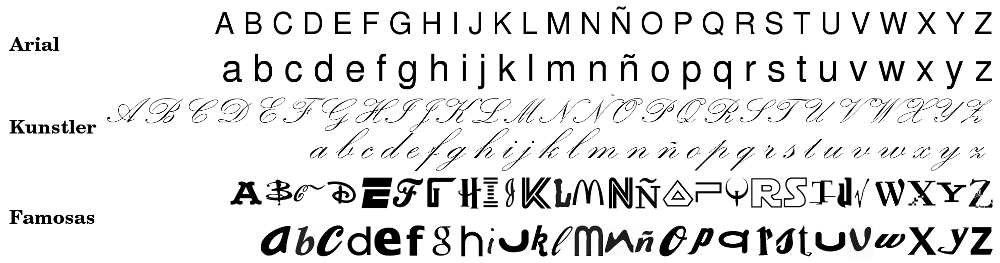
\includegraphics[scale=.20]{graficos/letras.png}
\end{figure}

\end{columns}
\end{frame}

%Gosselin
\begin{frame}
 \frametitle{Gosselin}
 \begin{columns}[t]
  \column{.5\textwidth}
   \begin{block}{Bubbles (GosselinySchyns)}
    \begin{itemize}
    \item Cookbook de cualquier experimento con Bubbles
    \item Bubbles locas
    \end{itemize}
   \end{block}
  \column{.5\textwidth}
   \begin{figure}
   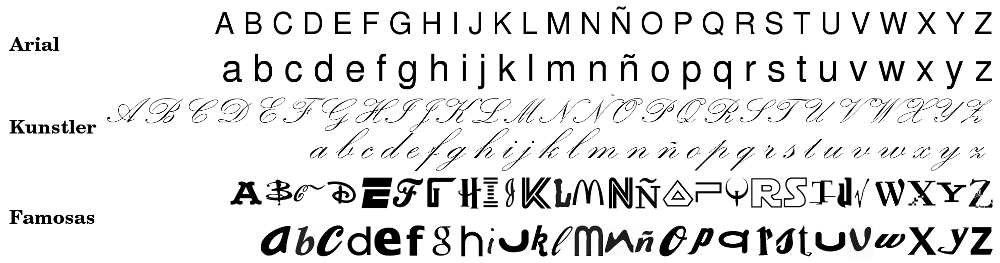
\includegraphics[scale=.20]{graficos/letras.png}
   \end{figure}
  \end{columns}
\end{frame}


%Fiset
\begin{frame}
\frametitle{Feature for Identification of Uppercase and Lowercase Letters (Fiset et al., 2008)}

\begin{columns}[t]
 \column{.5\textwidth}
  \begin{figure}
    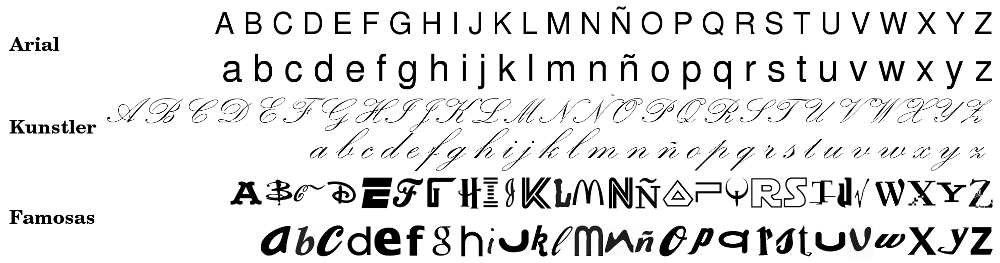
\includegraphics[scale=.10]{graficos/letras.png}
  \end{figure}
  \column{.5\textwidth}
   \begin{figure}
    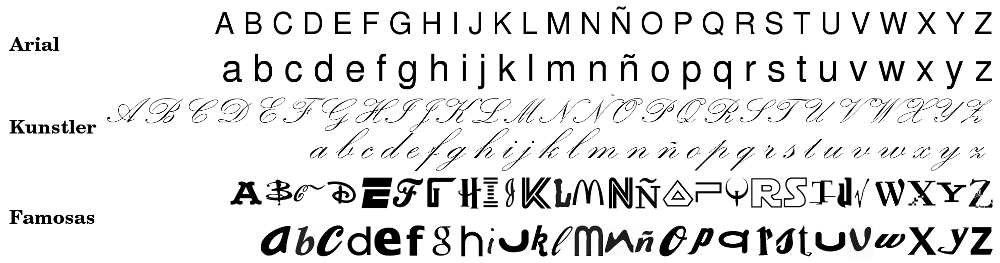
\includegraphics[scale=.1]{graficos/letras.png}
   \end{figure}
\end{columns}

\end{frame}



\subsection{Diseño}
%Sujetos+estímulos
\begin{frame}
\frametitle{Est\'imulos}
\begin{figure}
 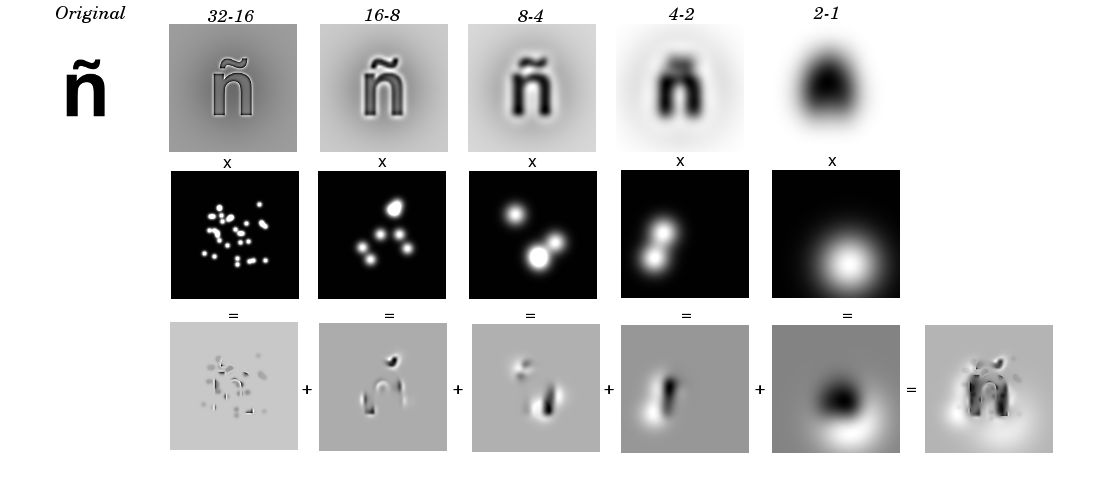
\includegraphics[width=\textwidth]{graficos/estimulofinal.png}
\caption{Armado del est\'imulo final}
\end{figure}
\end{frame}

\end{document}
